% Please do not change the document class
\documentclass{scrartcl}

% Please do not change these packages
\usepackage[hidelinks]{hyperref}
\usepackage[none]{hyphenat}
\usepackage{setspace}
\doublespace

% You may add additional packages here
\usepackage{amsmath}
\usepackage{graphicx}
\graphicspath{ {Figures/} }

% Please include a clear, concise, and descriptive title
\title{Usability Analysis}

% Please do not change the subtitle
\subtitle{COMP140 - Usability Analysis}

% Please put your student number in the author field
\author{1507866}

\begin{document}
	
\maketitle


\section{Introduction}
This report will analyse the COMP140 hardware hacking controller using the heuristic analysis method suggested by Nielsen \cite{HeuristicEvaluation}.


\section{Heuristics}
The heuristics that were used were designed by Nielsen:

\begin{itemize}
	\item Visibility of system status
	\item Match between system and the real world
	\item User control and freedom	
	\item Consistency and standards
	\item Error prevention
	\item Recognition rather than recall
	\item Flexibility and efficiency of use
	\item Aesthetic and minimalist design
	\item Help users recognize, diagnose, and recover from errors	
	\item Help and documentation \cite{NNG}
\end{itemize}

However Nielsen's heuristics are not specific to games. Pinelle \textit{et al} has designed heuristics that are game specific. The heuristics used here are relating to game controls such as clumsy input scheme and command sequences being too complex \cite{Pinelle}.

\section{The Controller}

\begin{figure}[h]
	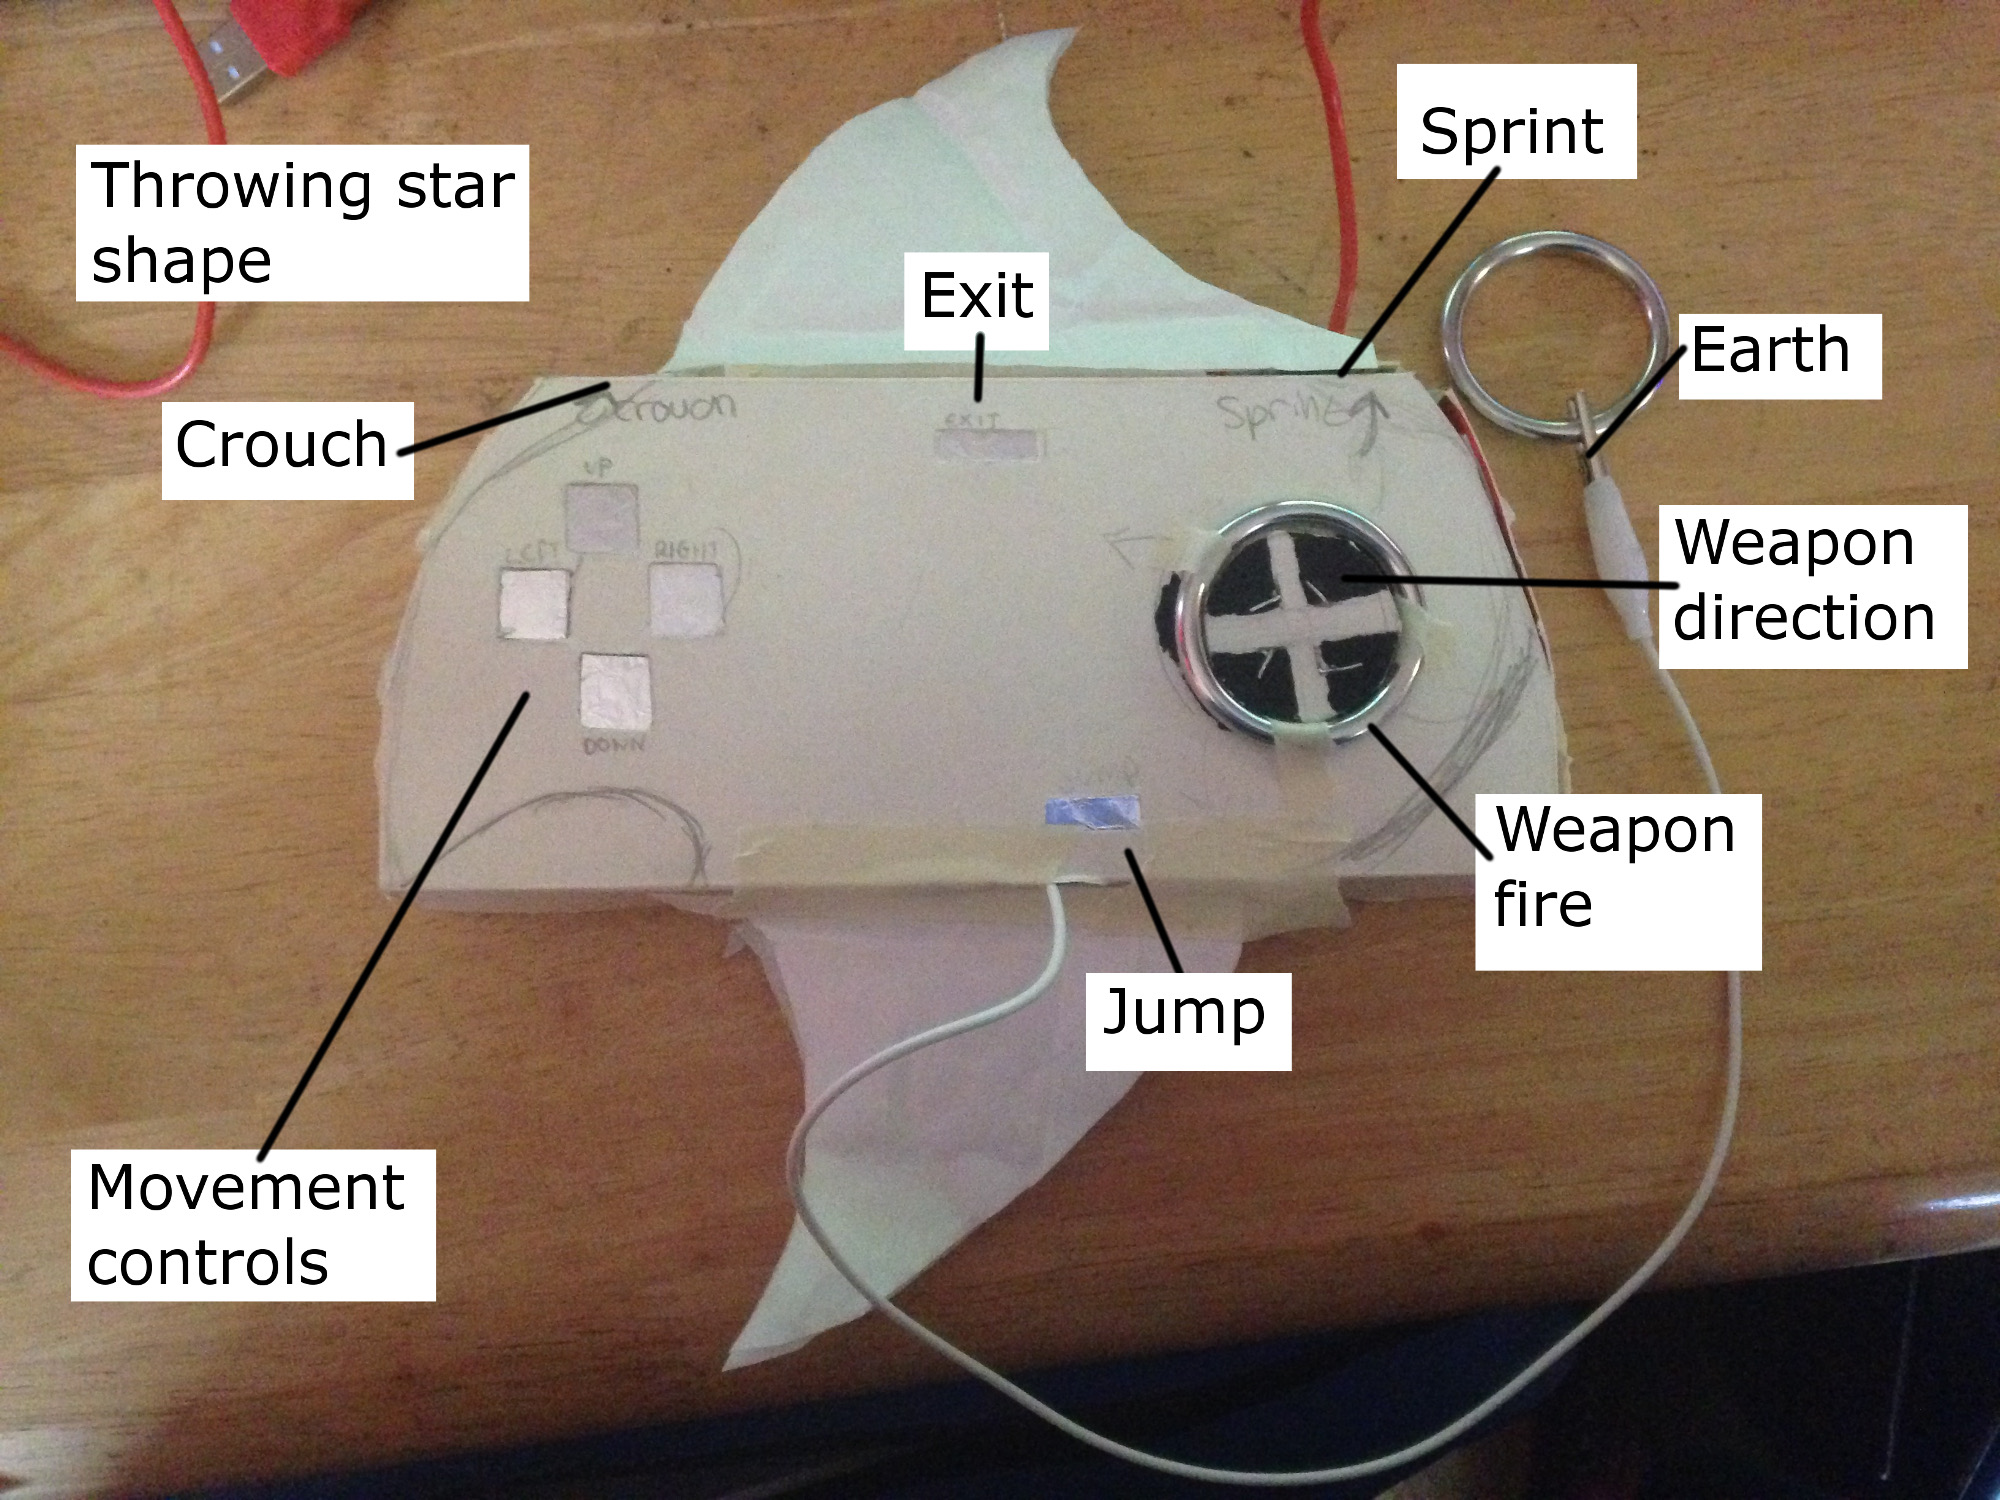
\includegraphics[width=1.0\linewidth]{Controller.jpg}
	\caption{ The controller.}
\end{figure}
Figure 1 shows the controller, it is shaped like a throwing star to fit the theme of the game it was designed for. It is designed for younger children that are more likely to be interested in different shaped controllers.

\section{Two Improvements}

The first issue with the controller is the aesthetic and minimalist design. The shape means that one side will be shaped similarity to a controller such as the PS4 controller, this side should be easy to grip and use. However the other side curves upwards and may be hard to grip. This may lead to the buttons on that side of the controlled being harder to use. Also the change in shape may mean that the controller is uncomfortable to use for extend periods of use. A possible improvement could be to alter the shape of the controller to give it two hand grips.

\begin{figure}[h]
	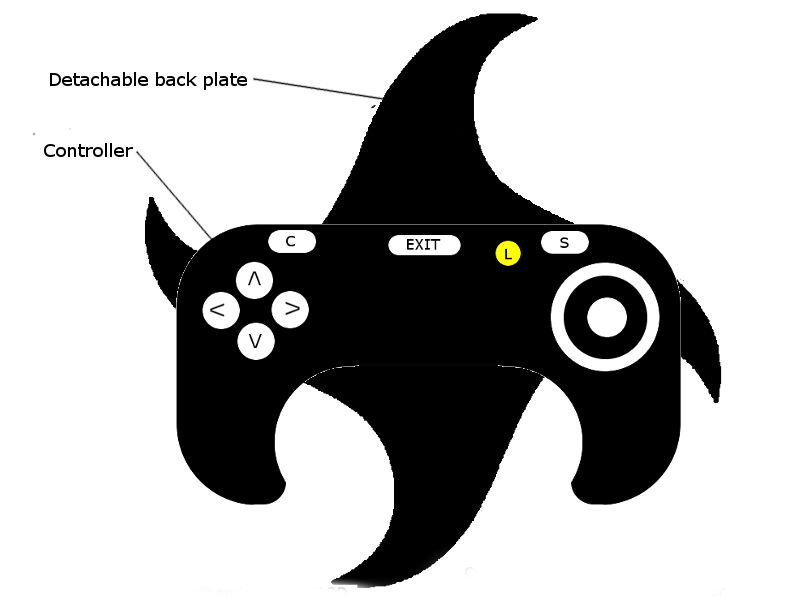
\includegraphics[width=1.0\linewidth]{Improved_design.png}
	\caption{Potential improved design .}
\end{figure}

 Figure 2 shows a possible alternate design that has two hand grips making it easier to hold. The throwing star shape is also removable meaning it can be taken off if it is causing discomfort. This also allows for alternate shapes to be attached to the controller for use with other games. 

Another issue is the visibility of system status, the controller should inform the user of the system status. Currently there is no indicator as to whether the controller is functioning correctly. The MakeyMakey kit has an LED to indicate whether it is powered on, the controller casing could be adapted to make this LED visible so the user. The MakeyMakey also has the functionality to add another LED that will flash when a button is pressed. An LED could be added to the controller to test whether the buttons are all functional. These two improvements will inform the user of the system status. 
\break
\section{Conclusion}
Nielsen says that it is difficult for an individual to find all the usability issues  \cite{HeuristicEvaluation}. Therefore there are likely to be more issues with the controller that would be found if it was analysed by more people. However making the two improvements will improve the usability of the controller.


\bibliographystyle{ieeetr}
\bibliography{comp140}
	
\end{document}
